\documentclass[12pt]{article}

\usepackage[english]{babel}
\usepackage[utf8]{inputenc}
\usepackage{fancyhdr}
\usepackage[margin=1in]{geometry}
\usepackage{amsmath}
\usepackage{amsfonts}
\usepackage{amssymb}
\usepackage{scrextend}
\usepackage{enumitem}
\usepackage{tikz}
\usepackage{pgfplots}
\usepackage{multirow,array}
\usepackage{float}
\usepackage{graphicx}


\begin{document}

%\vspace*{\stretch{1.0}}
\begin{center}
 	\Large\textbf{(Draft) Multi-market simulation}\\
 	\large\textit{Saketh Aleti}
\end{center}
\rule{\textwidth}{1pt}

	
\section{Market Model}	

\subsection{Definitions}

Suppose we have a system of supply and demand curves for $n$ commodities; each curve is a function of the prices of the other commodities. So, we have:
\begin{subequations}
\begin{align}
\textbf{Supply: } & Q_{s,i} = \alpha_{s,i} + \beta_{s,i,1} P_1 + ... + \beta_{s,i,n} P_n				\\
\textbf{Demand: } & Q_{d,i} = \alpha_{d,i} + \beta_{d,i,1} P_1 + ... + \beta_{d,i,n} P_n	
\end{align}
\end{subequations}

Now, suppose that this system is in equilibrium at time $t = 0$ where $P_0$ and $Q_0$ are vectors representing the equilibrium price and quantity. We then introduce a predefined shock, ${\alpha_{shock,i}} $, to each supply curve and define $ \alpha_{s,i}' = {\alpha_{s,i}}+ {\alpha_{shock,i}} $. Thus, the new supply curve is: 
\begin{equation}
\textbf{New Supply: }  Q_{s,i} = \alpha_{s,i}' + \beta_{s,i,1} P_1 + ... + \beta_{s,i,n} P_n  \tag{1c}
\end{equation}

Suppose this shock occurs at time $t=1$; at this moment, the price and quantity are not in equilibrium. We find the equilibrium price and quantity by solving:
$$ \alpha_{s,i}' + \beta_{s,i,1} P_1 + ... + \beta_{s,i,n} P_n = \alpha_{d,i} + \beta_{d,i,1} P_1 + ... + \beta_{d,i,n} P_n$$
Now, we use the following definitions for simplicity:
$$ 
\alpha=\begin{bmatrix}
 	\alpha_{s,1}' - \alpha_{d,1} \\
 	\vdots\\
 	\alpha_{s,n}' - \alpha_{d,n}
\end{bmatrix} 
,\quad
\beta=\begin{bmatrix}
\beta_{d,1,1} - \beta_{s,1,1} & \dots & \beta_{d,1,n} - \beta_{s,1,n} \\
\vdots & \ddots & \vdots \\
\beta_{d,n,1} - \beta_{s,n,1} & \dots & \beta_{d,n,n} - \beta_{s,n,n}
\end{bmatrix} 
,\quad
P=\begin{bmatrix}
P_1 \\
\vdots\\
P_n
\end{bmatrix} 
,\quad
Q=\begin{bmatrix}
Q_1 \\
\vdots\\
Q_n
\end{bmatrix} 
$$
We can then simplify the former equation into $\beta P = \alpha$ and solve to give us the equilibrium price; the equilibrium quantity then follows from a substitution into equation (1b) or (1c). 

\subsection{Dynamics}

Suppose, however, that all markets did not simultaneously fall into equilibrium. That is, assume the producers for each commodity set prices simultaneously for their commodity's market but not for the entire market consisting of all commodities. Then, after the first supply shock at time $t=1$, we initially solve the following system:
\begin{align*}
Q_{1} &= \alpha_s' + \beta_s P_1 \\
P_{1}& = \alpha_d  + diag(\beta_d) P_1
\end{align*}
Here, $diag(\beta_d)$ refers to a matrix consisting only of the diagonal elements of $B_d$. Solving this system then results in a new non-equillibrium price that has yet to take into account shifts in demand due to cross elasticities.


Assume that each producer $i$ does not expect the market's prices for all commodities but his own to change in the next timestep. Doing so essentially means he best responds to the demand curve for the market at time $t$. The demand curve for commodity $i$ is defined as:

\begin{align*}
Q_{t,i} &= \alpha_{d,i} + \beta_d P_t \\
&= \alpha_{d,i} + \sum_{j \neq i} \beta_{d,j} P_{t,j} + \beta_{d,i} P_{t,i}
\end{align*}

The term $\beta_{d,j}$ refers to column $j$ of $\beta_d$.

 Then, at each time step, the producer solves:
\begin{align*}
Q_{t} &= \alpha_d + \beta_d P_t \\
P_{t+1}& = \beta_s^{-1} (Q_{t} - \alpha_s') \\
Q_{t+1} &= \alpha_s' + \beta_s P_{t+1}
\end{align*}
Here, at each timestep, producers of commodity $i$ assume that the demand curve will not change in the next timestep; hence, they implicitly assume the prices of other commodities will remain the same in the next timestep. Since all producers make this assumption, the demand curve in the next timestep does not reach equilibrium due to cross price elasticities. However, it does approach the true demand curves for all goods in equilibrium. Iterating through this process where $t \to \infty$ results in the system reaching equilibrium.   \\

To find the steady-state, we first transform this problem into a linear differential equation. So, we begin by computing the change in price at each time $t$:
\begin{align*}
{\partial P}/{\partial t} &= P_{t+1} - P_t 		     \\
&= \beta_s^{-1} (Q_{t} - \alpha_s) - P_t				 \\
&= \beta_s^{-1} \alpha  + \beta_s^{-1} \beta_d P_t - P_t \\
&= \beta_s^{-1} \alpha  + (\beta_s^{-1} \beta_d - I) P_t
\end{align*}

From this, it follows that the steady-state is achieved when the change in price with respect to time is 0; let the steady-state solution be denoted as $P^*$. Therefore, setting the equation equal to zero, we have:

$$(\beta_s^{-1} \beta_d - I) P^* = -\beta_s^{-1} \alpha$$

To visualize this, the following graph shows the movement of the prices of two commodities towards the equilibrium. In the background is the vector field for this diff eq. The initial point is $P_{t=0}^T = (1,2)$ which converges to the equilibrium $(0.875,1.810)$.

\begin{center}
	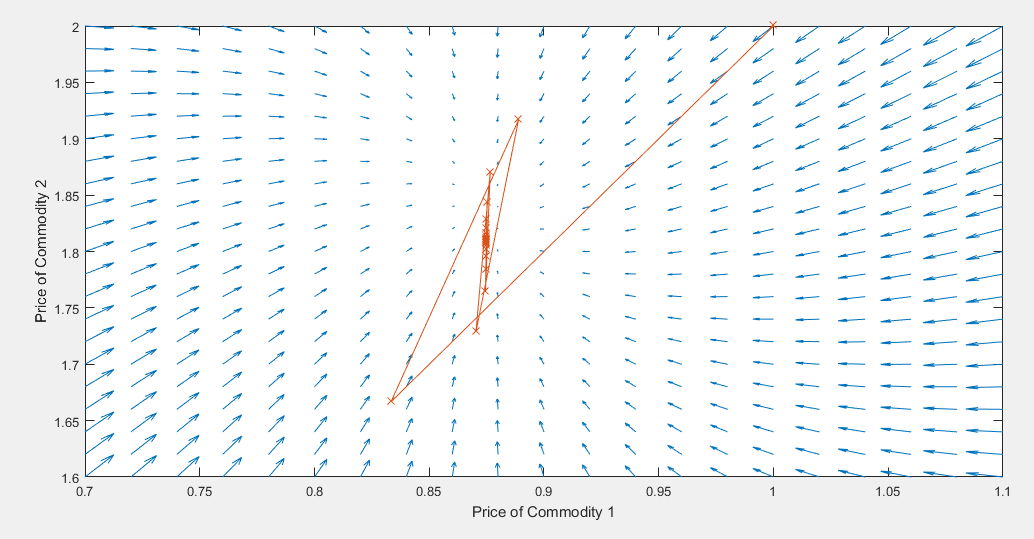
\includegraphics[scale = 0.5]{figures/vector_field}
\end{center}

However, the existence of an equilibrium point for this system does not necessarily imply that the prices will converge. For example, suppose we have the case where:

$$| P'_t | \geq | P'_{t-1} | $$

Here, $P'_t$ refers to the change in price at time $t$. This case is illustrated below, in a different system, where $P_0$ is marked by the red circle. Note that the vector field shows convergence, but the prices by increasingly larger amounts. 

\begin{center}
	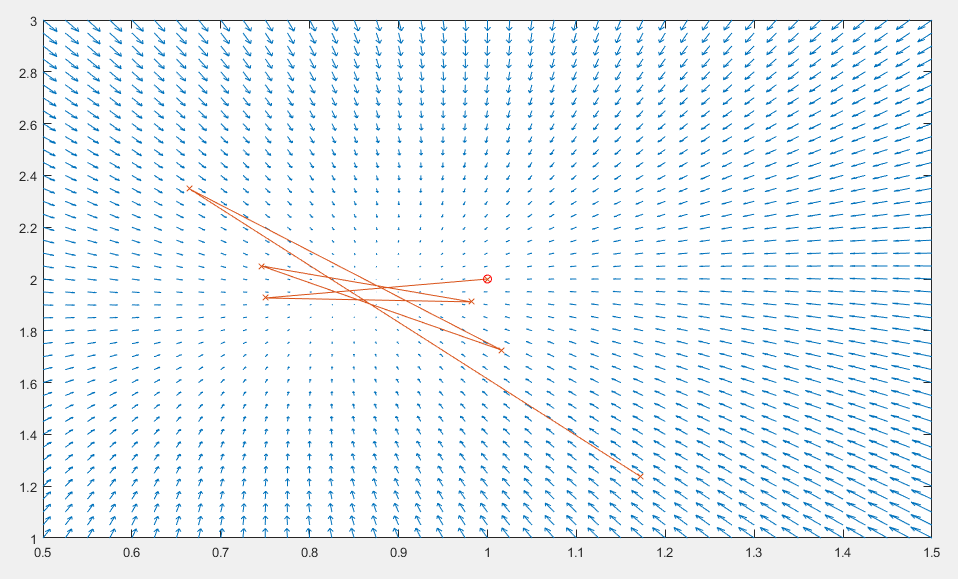
\includegraphics[scale = 0.5]{figures/vector_field2}
\end{center}

We see that, rather than converging, prices are unstable actually diverge in this system. The equilibrium to the system, if all equations are instead solved simultaneously, is simply $(0.868,1.944)$. Yet, this equilibrium is only stable if it is reached precisely. If we take the system at equilibrium and shift prices by a very small amount, the system again diverges. We can see this in the example below; the initial price was set to be very close but not exactly equal to the equilibrium

\begin{center}
	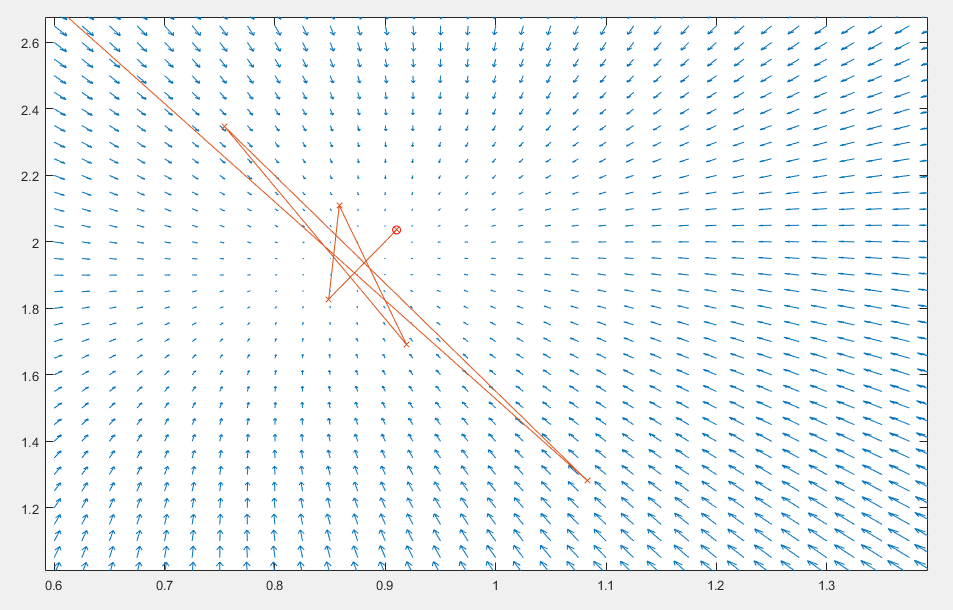
\includegraphics[scale = 0.5]{figures/vector_field3}
\end{center}
. 

\end{document}